\section{DoA and NCM estimation}
\label{sec:doa_ncm_estimation}

A minimization problem must be constructed, given the desire to find the most appropriate values for the DoA $\Theta$ and for the variances. We define a frequency-dependent cost function as
\begin{equation}
	\label{eq:sec3:cost_function}
	J\pts{\Corr*{\bvy}(\bvsi,\Theta)}[k] = \fnorm{\Corr*{\bvy}[k] - \Corr{\bvy}[k]}^2
\end{equation}
where $J(\Corr*{\bvy}(\bvsi,\Theta)[k])$ is implicitly a function of $\Theta$, and the variances $\var{x_1}$ through $\var{v_1}$. We let $\bvsi = \left[\var{x_1},~\var{p_1},~\var{\gamma_1},~\var{v_1}\right]$ be a vector of the unknown variances, and denote $R_{\bvy;\bvj}$ as the $[i,j]$-th element of a generic $\bv{R}$ (with $\bvj = [i,j]$). With this, we have
\begin{equations}{eq:sec3:cost_function_eachfreq}
	& J\pts{\Corr*{\bvy}(\bvsi,\Theta)} [k] = \\
	& \sum_{\bvj} \abs{\bts{\sum_{\bvz\in\sigs[k]} R_{\bvz;\bvj}[k] \var{z_1}[k]} - \pts{R_{\bvy;\bvj}[k] - \epsilon I_{\bvj}}}^2
\end{equations}
with $\sigs[k] = \cts{\bvx[k],\bvp[k],\bvga[k],\bvv[k]}$, and $\bvz$ generically symbolizing any of the variances. For simplicity, we denote $ \Corr{\bvy} - \epsilon\Id \equiv \Corr{\bvy,\epsilon}$.

By splitting the absolute value's calculation into the sum of real and imaginary components, \cref{eq:sec3:cost_function_eachfreq} can be modified into \cref{eq:sec3:cost_function_longform}, where the superscripts $\re$ and $\im$ indicate the real and imaginary parts of the value, respectively.

\begin{equation}
	\begin{split}
		J\pts{\Corr*{\bvy}(\bvsi,\Theta)} [k] 
		& = \sum_{\bvj}
		\pts{\bts{\sum_{\bvz\in\sigs[k]} \Re{R_{\bvz;\bvj}}[k] \var{z_1}[k]} - \Re{R_{\bvy,\epsilon;\bvj}}[k]}^2 \\
		& + \sum_{\bvj}
		\pts{\bts{\sum_{\bvz\in\sigs[k]} \Im{R_{\bvz;\bvj}}[k] \var{z_1}[k]} - \Im{R_{\bvy,\epsilon;\bvj}}[k]}^2
	\end{split}
	\label{eq:sec3:cost_function_longform}
\end{equation}

With the narrowband frequency-dependent cost function $J\pts{\Corr*{\bvsi,\Theta}}[k]$, we now define our broadband cost function $\cost{\bvSi,\Theta}$ as
\begin{equation}
	\label{eq:sec3:cost_function_broadband}
	\cost{\bvSi,\Theta} = \sum_{k} J\pts{\Corr*{\bvy}(\bvSi[k], \Theta)}[k]
\end{equation}
$\bvSi$ corresponds to a vector containing the variances for each frequency bin.

\subsection{Minimization on variances}
Physically, the variances must be strictly non-negative, and therefore a minimization problem would need to satisfy this condition; that is, $\bvsi[k] \geq \bv{0}\forall k$; this constraint is called the feasible region. We will employ the Lagrangian multiplier method \cite{rockafellar_lagrange_1993} to approach this problem. For such, we define the Lagrangian function $\lag(\bvsi,\Theta,\bvze,\bvmu)$ as
\begin{equation}
	\label{eq:sec3:lagrangian_function}
	\lag(\bvsi,\Theta,\bvze,\bvmu) = \cost{\Corr*{\bvy}(\bvsi,\Theta)[k]} - \tr{\bvze}\pts{\bvSi - \bvmu}
\end{equation}
with $\bvze$ being the Lagrange multiplier vector, and $\bvmu = \bts{\mu_x^2,\mu_p^2,\mu_\gamma^2,\mu_v^2}$ the slack variables (given the inequality constraint), with both $\bvze$ and $\bvmu$ being implicitly frequency-dependent. We denote $\pts{\bvSi\opt,\Theta\opt,\bvze\opt,\bvmu\opt}$ as the solution to the minimization problem, given by
\begin{equation}
	\label{eq:sec3:lagrangian_multiplier_eq}
	\bvSi^{\star},\Theta\opt,\bvze\opt,\bvmu\opt = \argmin_{\bvSi,\Theta,\bvze,\bvmu} \lag(\bvSi,\Theta,\bvze,\bvmu)
\end{equation}

Since $J\pts{\Corr*{\bvy}}$ for each frequency bin is independent from another bin, taking the derivative of the Lagrangian w.r.t. any variance $\var{z}[k]$ will result in
\begin{equation}
	\label{eq:sec3:partial_derivative_var-z}
	\pdv{\lag}{\var{z}[k]} = \sum_{\bvw\in\sigs[k]} A_{\bvw;\bvz}[k] \var{w}[k] - \zeta_{z}[k]
\end{equation}
where  $A_{\bvw;\bvz}$ is
\begin{equations}
	A_{\bvw;\bvz}[k]
	& = \sum_{\bvj} \Re{R_{\bvw;\bvj}}[k] \Re{R_{\bvz;\bvj}}[k] + \Im{R_{\bvw;\bvj}}[k] \Im{R_{\bvz;\bvj}}[k] \\
	%	& = \frac{1}{2} \sum_{\bvj} R_{\bvw;\bvj} {R_{\bvz;\bvj}}^* +{ R_{\bvw;\bvj}}^* R_{\bvz;\bvj}
\end{equations}
This derivative can be straightforwardly obtained from \cref{eq:sec3:cost_function_longform}. Differentiating the Lagrangian w.r.t. $\zeta_{z}[k]$ yields
\begin{equation}
	\label{eq:sec3:partial_derivative_xi-z}
	\pdv{\lag}{\zeta_{z}[k]} = \var{z}[k] - \mu_{z}[k]
\end{equation}
and w.r.t. $\mu_{z}[k]$ yields
\begin{equation}
	\label{eq:sec3:partial_derivative_mu-z}
	\pdv{\lag}{\mu_{z}[k]} = 2\zeta_{z}\mu_{z}
\end{equation}

The variances which minimize the cost function from \cref{eq:sec3:cost_function_broadband} is one of the solutions where all derivatives in \cref{eq:sec3:partial_derivative_var-z,eq:sec3:partial_derivative_xi-z,eq:sec3:partial_derivative_mu-z} are zero. First we will solve the unconstrained variance minimization problem, then use this solution to achieve the optimal variance vector for the constrained problem, in the case where the global minimum isn't within the feasible region.

\subsubsection*{Unconstrained solution}
Since each variance depends only on the variances in its own bin, our global minimization problem over all $4K$ variances can be split into $K$ problems with $4$ variables each, and for each $k$ the (unconstrained) minimization can be written as
\begin{equation}
	\bvA[k] \bvsi[k] = \bvq[k]
\end{equation}
where
\begin{subgather}{subeqs:sec3:definition_bvA_bvq}
	\bvA[k] = \begin{bmatrix}
		A_{\bvx;\bvx}[k] & A_{\bvp;\bvx}[k] & A_{\bvga;\bvx}[k] & A_{\bvv;\bvx}[k] \\
		A_{\bvx;\bvp}[k] & A_{\bvp;\bvp}[k] & A_{\bvga;\bvp}[k] & A_{\bvv;\bvp}[k] \\
		A_{\bvx;\bvga}[k] & A_{\bvp;\bvga}[k] & A_{\bvga;\bvga}[k] & A_{\bvv;\bvga}[k] \\
		A_{\bvx;\bvv}[k] & A_{\bvp;\bvv}[k] & A_{\bvga;\bvv}[k] & A_{\bvv;\bvv}[k]
	\end{bmatrix} \label{subeq:sec3:definition_bvA}\\
	\bvq[k] = \begin{bmatrix}
		A_{\bvy;\bvx}[k] + \zeta_{x}[k]\\
		A_{\bvy;\bvp}[k] + \zeta_{u}[k]\\
		A_{\bvy;\bvga}[k] + \zeta_{\gamma}[k]\\
		A_{\bvy;\bvv}[k] + \zeta_{v}[k]
	\end{bmatrix} \label{subeq:sec3:definition_bvq}
\end{subgather}
and therefore the solution to the unconstrained problem is
\begin{equation}
	\label{eq:sec3:solution_unconstrained-minim_bvsi}
	\bvsi^{\star}[k] = \inv{\bvA}[k] \bvq[k]
\end{equation}

This result doesn't necessarily respect the constraint $\bvsi[k] \geq \bv{0}$, as neither $\inv{\bvA}[k]$ nor $\bvq[k]$ are guaranteed to be positive vectors.

\subsubsection*{Constrained solution}
For each of the signals (generically $z[l,k]$), from \cref{eq:sec3:partial_derivative_mu-z} we have two options: either $\zeta_z[k] = 0$, meaning the constraint is inactive and the minimization is unrestricted in $z$; or $\mu_z[k] = 0$, which from \cref{eq:sec3:partial_derivative_xi-z} implies that ${\var{z}[k] = 0}$, meaning the constraint is active. The unconstrained problem's process can be adapted to find the restricted problem's solution through the following:

First, the unconstrained problem is solved (with \cref{subeqs:sec3:definition_bvA_bvq,eq:sec3:solution_unconstrained-minim_bvsi}), and we test if all variances respect the constraint. If so, the global minimum satisfies the necessary conditions, and the solution was found.

If any variance is negative, we test all combinations of active/inactive constraints among the negative variances of this global minimum, check which combinations respect the constraints, and from these we choose the one that minimizes the cost function. A more in-depth explanation on this analysis is in \cref{app:appC:active-inactive_analysis}, with all necessary proofs in\cref{thm:no-constraints_global_min_positive_values,thm:constrained_min_boundary}.

Notice that $\var{z} = 0$ when the $z$-th constraint is active. This removes one of the minimization variables, and its respective row and column in $\bvA$, as well as entries in $\bvq$ and $\bvsi$, can be disregarded.

Since we achieve the solution to this problem through at most $16$ matrix inversions, we say that a quasi-linear solution to the variances minimization can be achieved, not relying on iterative processes. This process is repeated for all $k$ bins, achieving the $4K$ solutions for the variances.

This minimization solves only for $\bvSi$, treating $\Theta$ as a constant. Since any element of $\bvA$ and $\bvq$ that corresponds to $\bvp$ depends on $\Theta$, so do the achieved solutions. That is, for each direction $\Theta$ we can find a solution on $\bvSi$ which minimizes the error between $\Corr*{\bvy}$ and $\Corr{\bvy}$, satisfying the constraints. Therefore, it is necessary to minimize $\cost{\Corr*{\bvy}(\bvsi)}$ with respect to the DoA.

\subsection{Minimization on DoA}

By definition, $R_{\bvp;\bvj}(\theta_b,\phi_b)$ interfering source's correlation between any two sensors, and can be written as
\begin{equation}
	R_{\bvp;\bvj}(\theta_b,\phi_b) = e^{-\j \frac{2\pi f}{c} r_{\bvj} \cos\pts{\theta_b - \psi_{\bvj}} \cos\pts{\phi_b - \lambda_{\bvj}}}
\end{equation}
where $r_{\bvj}$, $\psi_{\bvj}$ and $\lambda_{\bvj}$ are the relative distance, azimuth, and elevation between the $i$th and $j$-th sensors.

The derivatives of the cost function in \cref{eq:sec3:lagrangian_function} w.r.t. $\theta_b$ and $\phi_b$ are, respectively,
\begin{equation}
	\label{eq:secA:pdv_lagrangian_theta}
	\pdv{\cost}{\theta_b} = -\frac{4\pi f}{c}\sum_{\bvj} f_1(\theta_b,\phi_b,\bvj) G(\theta_b,\phi_b,\bvj)
\end{equation}
\begin{equation}
	\label{eq:secA:pdv_lagrangian_phi}
	\pdv{\cost}{\phi_b}   = -\frac{4\pi f}{c}\sum_{\bvj} f_2(\theta_b,\phi_b,\bvj) G(\theta_b,\phi_b,\bvj)
\end{equation}
in which
\begin{subgather}{eqs:sec3:parameters_pdv_lagrangian_dirs}
	f_1(\theta_b,\phi_b,\bvj) = \sin\pts{\theta_b - \psi_{\bvj}} \cos\pts{\phi_b - \lambda_{\bvj}} \\
	f_2(\theta_b,\phi_b,\bvj) = \cos\pts{\theta_b - \psi_{\bvj}} \sin\pts{\phi_b - \lambda_{\bvj}} \\
	%G(\theta_b,\phi_b,\bvj) = -r_{\bvj} \sum_{k} \alpha[k] \imag{ \pts{\hat{R}_{\bvy;\bvj}[k] - R_{\bvy;\bvj}[k]}^* R_{\bvp;\bvj}(\theta_b,\phi_b)[k] }
	G(\theta_b,\phi_b,\bvj) = r_{\bvj} \sum_{k} \var{p_1}[k] \imag{ \bar{R}^*_{\bvj}[k] R_{\bvp;\bvj}(\theta_b,\phi_b)[k] } 
\end{subgather}
where $\bar{R}_{\bvj}[k] = R_{\bvx;\bvj}[k] + R_{\bvga;\bvj}[k] + R_{\bvv;\bvj}[k] - R_{\bvy,\epsilon;\bvj}[k]$. From now the $\nfrac{4\pi f}{c}$ term will be ignored (except for $f = 0$), as it is a positive constant and doesn't affect neither the zeros nor the sign of the derivatives.

We now consider the following properties:
\begin{itemize}
	\item For any diagonal element, $r_{[i,i]} = 0$;
	\item For any element $-\bvj \equiv [j,i]$:
	\begin{itemize}
		\item $r_{-\bvj} = r_{\bvj}$
		\item $\psi_{-\bvj} = \psi_{\bvj} + \pi$
		\item $\lambda_{-\bvj} = -\lambda_{\bvj}$
		\item $G(\theta_b,\phi_b,-\bvj) = -G(\theta_b,\phi_b,\bvj)$
	\end{itemize}
\end{itemize}
With these, we have that
\begin{subgather}
	f_1(\theta_b,\phi_b,-\bvj) = -\sin(\theta_b - \psi_{\bvj}) \cos(\phi_b + \lambda_{\bvj}) \\
	f_2(\theta_b,\phi_b,-\bvj) = -\cos(\theta_b - \psi_{\bvj}) \sin(\phi_b + \lambda_{\bvj})
\end{subgather}
and therefore, by gathering the $\bvj$ and $-\bvj$ terms in the summations of \cref{eq:secA:pdv_lagrangian_theta,eq:secA:pdv_lagrangian_phi}, through trigonometric properties they can be simplified to
\begin{subgather}{eqs:sec3:pdv_cost_angles_simplified}
	\pdv{\cost}{\theta_b} = 2\cos\pts{\phi_b}\sum_{\substack{\bvj=[i,j]\\i<j}} \sin\pts{\theta_b - \psi_{\bvj}} \cos\pts{\lambda_{\bvj}} G(\theta_b,\phi_b,\bvj) \label{eqs:sec3:pdv_cost_angles_simplified:subeq1}\\
	\pdv{\cost}{\phi_b} = 2\sin\pts{\phi_b}\sum_{\substack{\bvj=[i,j]\\i<j}} \cos\pts{\theta_b - \psi_{\bvj}} \cos\pts{\lambda_{\bvj}} G(\theta_b,\phi_b,\bvj) \label{eqs:sec3:pdv_cost_angles_simplified:subeq2}
\end{subgather}

Both $\pdv{\lag}{\theta_b}$ and $\pdv{\lag}{\phi_b}$ are heavily non-linear, and therefore a straightforward solution can't be easily found. However, as this is an unconstrained minimization problem with restricted domain, an approximate solution can be achieved through methods such as iterative minimization or an exhaustive search.

We propose the use of the gradient descent technique, as both the function and its derivatives are accessible. Since the gradient descent requires an initial guess, our minimization process can either use a multi-initialization step, or a previously estimated DoA.

\subsubsection*{Source-tracking procedure}

When defining the problem, we assumed that the sources are stationary, which implies that the correlation matrices and steering vectors are independent of $l$. It is trivial to generalize the shown procedures to be done every frame, or every couple of frames. This, coupled with the necessity of an initial guess for $\Theta$ in the minimization process, allows for a source-tracking method within the NCM and DoA estimation procedure, as long as the source isn't rapidly moving.

Formally, we can use an estimate from a previous time frame as the current frame's initial guess, $\Theta_0[l] = \bar{\Theta}[l-\Delta]$. If the source's position change rapidly, a multi-initialization is possibly necessary to ensure that the global minimum is achieved.

\subsection{Approximations and specific-array considerations}
\label{subsec:sec3:approximations_specific-array_considerations}

Although the established process is generic and works with any sensor configuration, the results can be simplified in some scenarios.

\subsubsection*{General approximation}

From \cref{eqs:sec3:pdv_cost_angles_simplified}, it is easy to see that $\phi_b = 0\dg$ leads to a null in $\npdv{\cost}{\phi_b}$, and $\phi_b = 90\dg$ a null in $\npdv{\cost}{\theta_b}$. However, these nulls are due to the geometric construction and choice of variables, and unrelated to the DoA estimation procedure. They are also linked to points of maxima in the respective variable, thus being unhelpful in the cost function's minimization. Therefore, we postulate it is safe to assume that they can be ignored when calculating the derivative, as they slow down the minimization in the best case, and actively interfere and lead to false results in the worst-case.

That is, we say that
\begin{subgather}
	\pdv{\cost}{\theta_b} \approx \sum_{\substack{\bvj=[i,j]\\i<j}} \sin\pts{\theta_b - \psi_{\bvj}} \cos\pts{\lambda_{\bvj}} G(\theta_b,\phi_b,\bvj) \\
	\pdv{\cost}{\phi_b} \approx \sum_{\substack{\bvj=[i,j]\\i<j}} \cos\pts{\theta_b - \psi_{\bvj}} \cos\pts{\lambda_{\bvj}} G(\theta_b,\phi_b,\bvj)
\end{subgather}
is a sufficiently good approximation of the derivatives. In a case where $\phi_b = 0\dg$ or $\phi_b = 90\dg$ would minimize the cost function, they would also be roots in this new approximation.

\subsubsection*{Planar arrays}
If one is working with a planar array (be it linear, concentric, or any other planar arrangement), without loss of generality we can assume that $\psi_{\bvj} = 0 \forall \bvj$ (as a change of coordinate system can be applied to achieve this). Therefore, the $\cos(\lambda_{\bvj})$ term in both \cref{eqs:sec3:pdv_cost_angles_simplified:subeq1,eqs:sec3:pdv_cost_angles_simplified:subeq2} can be treated as a constant and ignored.

\subsubsection*{Linear arrays}

One useful consideration for the linear array case is its cylindrical symmetry. Given a direction $(\theta,\phi)$, there exists another direction $(\theta',0)$ such that their steering vectors are identical. It is easy to see that
\begin{equation}
	\theta' = \arccos\pts{\cos(\theta) \cos(\phi)}
\end{equation}
achieves this result. We thus assume that $\phi_b = 0$, and the DoA estimation is reduced to a single variable. 

Furthermore, the azimuth for all sensors is constant as well, and we can safely assume $\psi_{\bvj} = 0 \forall \bvj$ (again, through a change of coordinate system). Thus the $\sin(\theta_b)$ is independent of $\bvj$ and can be factored; not only that, but it will also be ignored, as it is related to the chosen coordinate system and a constant. With these assumptions and considerations in mind, we have
\begin{equation}
	\pdv{\cost}{\theta_b} \approx \sum_{\substack{j=[i,j]\\i<j}} G(\theta_b,0,\bvj)
\end{equation}

\subsection{Minimization scheme}

Being able to minimize the cost function in $\bvsi$ and $\Theta$, the global minimization scheme is as follows:
\begin{enumerate}
	\item Get an initial estimate $\Theta_0$. This is done via a random guess, using a direction from a previous time, or through multi-initialization.
	\item Use the active/inactive analysis to minimize the cost function $\bvsi$. Note that if the unconstrained minimization results in a valid vector of variances, the other combinations don't need to be tested.
	\item Check if derivatives with respect to $\theta_b$ and $\phi_b$ are within a desired threshold:
	\begin{enumerate}
		\item If not, go back to step 2, with updated $\theta_b$ and $\phi_b$ using a gradient descent method;
		\item If yes, break, and return the estimated parameters.
	\end{enumerate}
	\item Construct the NCM $\Corr{\bveta}$ as in \cref{eq:def_NCM_Corr-bveta}.
\end{enumerate}

The active-inactive analysis on $\bvsi[k]$ has to be repeated for each iteration of the minimization on $\Theta$, since for one direction the constraints have to be active, but not for a different neighboring direction.

%{\ieee
%Generally, it is clear that both derivatives' nulls can be achieved if (and only if) $D_1(\theta_b,\phi_b) = D_2(\theta_b,\phi_b) = 0$. Trivial zeros of these functions are achieved if $\cos\pts{\theta_b \pm \phi_b} = 0$, which are unrelated to our minimization process, and are due to the coordinate system's choice. We heuristically decide to ignore these two terms when calculating the derivative, as they in the best-scenario slow down the minimization, and in the worst-case can actively interfere and lead to wrong minimization results. That is, we let $\tD_1(\theta_b,\phi_b)$ and $\tD_2(\theta_b,\phi_b)$ be
%\begin{subgather}{eqs:sec3:D1_D2_without-cos}
%	\tD_1(\theta_b,\phi_b) = \sum_{\substack{\bvj=[i,j]\\i<j}} \sin\pts{\lambda_{\bvj} + \psi_{\bvj}} G(\theta_b,\phi_b,\bvj) \\
%	\tD_2(\theta_b,\phi_b) = \sum_{\substack{\bvj=[i,j]\\i<j}} \sin\pts{\lambda_{\bvj} - \psi_{\bvj}} G(\theta_b,\phi_b,\bvj)
%\end{subgather}
%and say
%\begin{subgather}{eqs:sec3:approx_cost_func_tD1_tD2}
%	\pdv{\cost}{\theta_b} \approx \tD_1(\theta_b,\phi_b) + \tD_2(\theta_b,\phi_b) \\
%	\pdv{\cost}{\phi_b} \approx \tD_1(\theta_b,\phi_b) - \tD_2(\theta_b,\phi_b)
%\end{subgather}
%
%\subsubsection*{Planar arrays}
%If one is working with a planar array (be it linear, rectangular, or any other planar arrangement), without loss of generality we can assume that $\psi_{\bvj} = 0 \forall \bvj$. This doesn't work with the approximations in \cref{eqs:sec3:D1_D2_without-cos,eqs:sec3:approx_cost_func_tD1_tD2}, as it would mean $\tD_1(\theta_b,\phi_b) = \tD_2(\theta_b,\phi_b)$ and therefore $\npdv{\cost}{\phi_b} = 0$. However, going back to \cref{eqs:sec3:pdv_cost_angles_simplified,eqs:sec3:D_funcs_pdv_cost_angles}, the derivatives can be instead simplified to
%\begin{subgather}
%	\pdv{\cost}{\theta_b} = 2\cos{\theta_b} \cos{\phi_b}\sum_{\substack{\bvj=[i,j]\\i<j}} \sin{\lambda_{\bvj}} G(\theta_b,\phi_b,\bvj) \\
%	%
%	\pdv{\cost}{\phi_b} = 2\sin{\theta_b} \sin{\phi_b}\sum_{\substack{\bvj=[i,j]\\i<j}} \sin{\lambda_{\bvj}} G(\theta_b,\phi_b,\bvj)
%\end{subgather}
%
%This formulation has trivial zeros if $[\theta_b,\phi_b] = [\pm\nfrac{\pi}{2}, 0]$ or $[\theta_b,\phi_b] = [0, \pm\nfrac{\pi}{2}]$, unrelated to our minimization process. By the same reasons as before, we choose to ignore these leading terms, which leads to
%\begin{equation}
%	\pdv{\cost}{\theta_b} = \pdv{\cost}{\phi_b} = 2\sum_{\substack{\bvj=[i,j]\\i<j}} \sin{\lambda_{\bvj}} G(\theta_b,\phi_b,\bvj)
%\end{equation}
%in which both derivatives are nulled with a single minimization.
%
%\subsubsection*{Linear arrays}
%If one is working with a linear array, the relative angles between any two sensors are the same; that is, $\psi_{\bvj} = \psi\forall\bvj$. In this scenario, the $\sin\lambda_{\bvj}$ is a constant, and since the objective is to find zeros of the derivatives, it can be disregarded. The edge case in which $\sin\lambda_{\bvj} = 0$ is another case of a coordinate-system null, and not a minimization null, and would only be harmful.
%
%Another consideration for the linear arrays is its cylindrical symmetry. Given a direction $(\theta, \phi)$, there exists a direction $(\theta',0)$ such that their steering vectors are identical. For such, it is easy to see that
%\begin{equation}
%	\theta' = \arccos(\cos(\theta)\cos(\phi))
%\end{equation}
%With this, the minimization can be reduced to a single angle, given that we can safely assume $\phi = 0$. In this case, $\cos(\phi)$ is maximized, and the optimization converges the fastest when minimizing for $\theta$.
%}
\subsection{Proposed model features}

The proposed estimation method exhibits several noteworthy properties. Its main appeal is its ability to jointly estimate the NCM and an interfering source's DoA, which theoretically improves performance in signal enhancement tasks. However, its current form allows the tracking of a single source, and wouldn't be suitable for multi-source conditions.

The DoA estimator is inherently broadband, leveraging information across multiple frequency bins to improve estimation robustness under reverberant or noisy conditions. Despite its broadband design, the method remains applicable to narrowband signals, offering flexibility across a range of applications. A further advantage lies in its ability to estimate both azimuth and elevation angles, thereby supporting full three-dimensional localization with two degrees of freedom.

The method's iterative nature naturally enables source tracking with the DoA being updated periodically, assuming the source position does not vary too rapidly. However, this iterative approach introduces some limitations. It is susceptible to local minima in the cost function, and there is no inherent guarantee that the global minimum corresponds to the true DoA. Furthermore, certain coordinate-induced ambiguities can lead to incorrect solutions, as addressed in \cref{subsec:sec3:approximations_specific-array_considerations}. The iterative optimization can also be computationally demanding, as the number of required steps varies and cannot be predetermined.

Given these characteristics, the proposed method should be adopted with consideration of its strengths and limitations. It offers significant advantages in environments dominated by a single directional interferer, particularly when robust beamforming are required. However, in dynamic or multi-source conditions, alternative or extended formulations may be more appropriate.

\subsection{Simulations for the DoA estimation}
\label{subsec:sec3:results_doa_estimation}

In this subsection, we will compare the proposed DoA estimator with the MUSIC algorithm \cite{gupta_music_2015}, comparing them for a wide range of situations.

\subsubsection*{MUSIC algorithm}
The proposed DoA estimation method will be fared against the traditional MUSIC algorithm \cite{gupta_music_2015}. For the MUSIC parameters, we assume the existence of a single source in the environment. Both the desired and undesired sources are in the same plane as the sensor array (such that its elevation is $0$). For the proposed DoA estimator, the initial guess is always $10\dg$ from the true source, simulating a spread-out multi-initialization process.

The MUSIC algorithm is commonly used for narrowband DoA estimation (although extensions to broadband have been proposed \cite{alrmah_extension_2011}), so it will be applied on all frequency bins, and two phasor-based methods will be used to achieve an estimate angle:

In the first one, a simple average will be taken across frequency, such that
\begin{equation}
	\bar{\theta}_{\music} = \angle\sum_{k} e^{\j\theta_{\music}[k]}
\end{equation}

In the second one, a weighted average will be taken, weighing each bin by its MUSIC spectrum, such that
\begin{equation}
	\bar{\theta}_{\wmusic} = \angle\sum_{k} p_{\wmusic}[k] e^{\j\theta_{w\music}[k]}
\end{equation}

\subsubsection*{Simulation scenarios}

All scenarios take place in a reverberant environment, with the room having dimensions $5\m\times5\m\times3\m$, and the array being positioned at $(1.5\m,1.5\m,1\m)$. The sensor array is an uniform rectangular array (URA) of dimensions $\sz{6}{2}$, and intersensor distance of $\delta=2\si{\centi\meter}$.

The spherical coordinate system's origin coincides with the center of the sensor array, and the desired source's azimuth is always $0\dg$. The correlated sources are positioned $1\m$ away from the origin, being 8 sources uniformly distributed in a circle. All sources' positions as described ahead are relative to the array's center. An example of a considered room layout is in \cref{fig:room_layout}.

\begin{figure}[t]
	\centering
%	\includesvg[width=0.8\linewidth]{sims_room_layout.svg}
	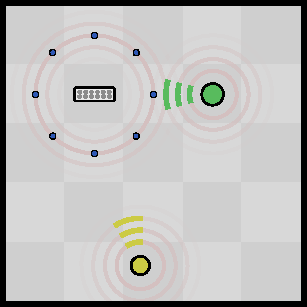
\includegraphics[width=0.8\linewidth]{input/drawings/sims_room_layout.pdf}
	\caption{Example of room layout. Desired source in green, undesired source in yellow, correlated sources in blue. Reverberations are shown as fading concentric red circles. Sensor array in gray, as a small rectangle.}
	\label{fig:room_layout}
\end{figure} 

The desired signal used is a male voice, the interfering signal a female voice, and the correlated sources are music. All signals and room impulse responses used were resampled to $16\si{\kilo\hertz}$. The time-frequency signals are obtained through the STFT, with $N = 64$ bins, and Hamming windows with overlap of $50\%$. The regularization parameter $\epsilon$ is set to $0.0001$, to ensure that a minimal white noise is considered. 

The amount of reverberation $\beta$, desired and undesired sources' distances $d_x$ and $d_u$, the undesired source's DoA $\theta_b$, as well as Signal-to-Interference Ratio (SIR) and Signal-to-Babble Ratio (SBR) are in \cref{tab:sec3:simulation_parameters}, totaling $486$ parameter combinations. These Signal-to-Noise Ratios (SNRs) are calculated between the desired signal's direct path signal, and the respective reverberant contaminant signal.

\begin{table}[!ht]
	\centering
	\renewcommand{\arraystretch}{1.4}
	\begin{tabular}{r l l l}
		Parameter & \multicolumn{3}{c}{Possible values} \\
		\hhline{====}
		$\beta$ & $0\ms$ & $150\ms$ & $500\ms$ \\
		$d_{x}$ & $50\cm$ & $100\cm$ & $150\cm$ \\
		$d_{u}$ & $50\cm$ & $100\cm$ & $200\cm$ \\
		$\theta_b$ & $20\dg$ & $50\dg$ & $80\dg$ \\
		SIR & $-3\db$ & $0\db $& $3\db$ \\
		SBR & $0\db$ & $5\db$ & $\sim$
	\end{tabular}
	\caption{Simulation parameters.}
	\label{tab:sec3:simulation_parameters}
\end{table}

In all tables, the bold result is the one that had the best performance in each metric, for each parameter value. The proposed method will be denoted NCM (red), the standard MUSIC will be MSC (green, dashed), and the weighted MUSIC will be called wMSC (in blue, dash-dotted).

\subsubsection*{Global results}

\begin{table}[t]
	\centering
	\renewcommand{\arraystretch}{1.4}
	\begin{tabular}{l l l l l l l}
		& \multicolumn{2}{c}{$20\dg$} & \multicolumn{2}{c}{$50\dg$} & \multicolumn{2}{c}{$80\dg$} \\
		\hhline{=======}
		& Avg. & Std. & Avg. & Std. & Avg. & Std. \\
		\hline
		NCM    & $7.93\dg$         & $11.08\dg$        & $\mbf{-0.49\dg}$  & $\mbf{2.92\dg}$   & $\mbf{-2.82\dg}$  & $\mbf{2.19\dg}$  \\
		MSC    & $\mbf{2.50\dg}$   & $\mbf{4.29\dg}$   & $-2.78\dg$        & $3.57\dg$         & $-8.14\dg$        & $3.28\dg$        \\
		wMSC   & $4.50\dg$         & $5.43\dg$         & $-1.28\dg$        & $5.15\dg$         & $-7.89\dg$        & $4.03\dg$
	\end{tabular}
	\caption{Global average and standard deviation for the prediction error results, for each undesired signal DoA.}
	\label{tab:sec3:error__each_DOA__total}
\end{table}

The results in \cref{tab:sec3:error__each_DOA__total} present the global average and standard deviation of the DoA estimation error for each interfering source direction, across $162$ simulation scenarios per angle. These serve as an overall snapshot of the estimator’s performance. For the $20\dg$ case, the MUSIC-based estimators (MSC and wMSC) outperform the proposed NCM method in both accuracy (mean error) and precision (standard deviation). However, in the $50\dg$ and $80\dg$ cases, the proposed NCM estimator exhibits superior performance across both metrics — modestly in the $50\dg$ case, and more decisively in the $80\dg$ scenarios.

\begin{figure}[t]
	\centering
	\hspace*{-1em}
	\tikzsetnextfilename{sec3-boxplot_doa_estim_global}
	\begin{tikzpicture}
		\begin{boxplot}[
			ylabel={Angle error ($\dg$)},
			xlabel={Undesired source's DoA ($\dg$)},
			xtick = {2, 6, 10},
			xmin = 0,
			xmax = 12,
			xticklabels={$20\dg$, $50\dg$, $80\dg$},
			xticklabel style = {align=center, font=\small},
			ymin=-18,
			ymax=18,
			ytick={-16, -8, ..., 16},
			legend to name = {BoxPlotErrorDg},
			legend style={
				legend columns=3,
				/tikz/every even column/.append style={column sep=1em}
			},
			legend cell align={left},]
			\addboxplot{1.03}{2.23}{7.93}{8.45}{15.97}[draw position=1][styleA]
			\addboxplot{-0.96}{-0.09}{2.50}{5.19}{7.87}[draw position=2][styleC]
			\addboxplot{-1.21}{-0.10}{4.50}{7.74}{13.78}[draw position=3][styleE]
			
			\addboxplot{-3.47}{-2.71}{-0.49}{0.41}{3.69}[draw position=5][styleA]
			\addboxplot{-7.22}{-4.97}{-2.78}{-0.85}{2.47}[draw position=6][styleC]
			\addboxplot{-7.15}{-3.76}{-1.28}{0.99}{5.46}[draw position=7][styleE]
			
			\addboxplot{-5.64}{-5.34}{-2.82}{-1.35}{-0.19}[draw position=9][styleA]
			\addboxplot{-12.56}{-10.26}{-8.14}{-5.61}{-4.19}[draw position=10][styleC]
			\addboxplot{-12.66}{-9.91}{-7.89}{-4.96}{-3.46}[draw position=11][styleE]
									
			\addplot[styleA] coordinates{(0, -1)};
			\addplot[styleC] coordinates{(0, -1)};
			\addplot[styleE] coordinates{(0, -1)};
			\addlegendentry{NCM};
			\addlegendentry{MSC};
			\addlegendentry{wMSC};
		\end{boxplot}
	\end{tikzpicture}
	\tikzsetnextfilename{sec3-boxplot_doa_estim_global_legend}
	\ppref{BoxPlotErrorDg}
	\caption{Error plot for the prediction error results, for each undesired signal DoA.}
	\label{fig:sec3:barplot_prediction_error}
\end{figure}

A complementary visualization is shown in \cref{fig:sec3:barplot_prediction_error}, where box plots illustrate the error distributions for each method, grouped by interfering source angle. The whiskers represent the $9$-th and $91$-st percentiles, while the box shows the interquartile range and median. The color scheme differentiates methods: red for the proposed NCM, green for MUSIC (MSC), and blue for weighted MUSIC (wMSC).

These visualizations reinforce the conclusions from \cref{tab:sec3:error__each_DOA__total}. At $50\dg$ and $80\dg$, the proposed method consistently yields both lower median error and reduced variability, indicating better precision and robustness. In contrast, at $20\dg$, the NCM estimator exhibits significantly higher variance, with wider tails in the error distribution. Nonetheless, the similarity in interquartile and whisker ranges across all methods suggests that core performance (excluding outliers) remains comparable, and the reduced accuracy of the NCM method at this angle is primarily due to more frequent extreme errors.

Further insight is gained by examining how often each method yields the lowest error across all $162$ simulation scenarios per frequency (as well as overall), as shown in \cref{tab:sec3:doa_estim_count_best}. The proposed NCM estimator dominates in the $50\dg$ and $80\dg$ conditions, while MUSIC and wMUSIC split the advantage in the $20\dg$ case, where NCM is clearly outperformed.

\begin{table}[!t]
	\centering
	\renewcommand{\arraystretch}{1.4}
	\begin{tabular}{l | l l l}
		& NCM & MSC & wMSC \\
		\hhline{====}
		$20\dg$ & 28 & 65 & 69 \\
		$50\dg$ & 119 & 26 & 17 \\
		$80\dg$ & 158 & 4 & 0 \\
		\hline
		Total & 303 & 95 & 88         
	\end{tabular}
	\caption{Number of best-result for each estimator, for each DoA.}
	\label{tab:sec3:doa_estim_count_best}
\end{table}

\subsubsection*{Results per DoA and per iSIR}

Additional depth is provided in \cref{tab:sec3:error__each_DOA__each_dist,tab:sec3:error__each_DOA__each_SIR}, which show the average and standard deviation of the angular estimation error for each combination of interfering DoA with either interfering distance or input SIR. Each result aggregates 54 simulations.

\begin{table}[!t]
	\centering
	\renewcommand{\arraystretch}{1.4}
	\begin{tabular}{l l l l l l l}
		\multicolumn{7}{c}{$20\dg$} \\
		\hhline{=======}
		& \multicolumn{2}{c}{$50\cm$} & \multicolumn{2}{c}{$100\cm$} & \multicolumn{2}{c}{$200\cm$} \\
		\hline
		& Avg. 				 & Std. 					& Avg. 				  & Std. 				 & Avg. 					& Std. \\
		\hline
		NCM    & $4.22\dg$         & $3.64\dg$         & $7.45\dg$         & $10.94\dg$        & $12.12\dg$        & $14.28\dg$       \\
		MSC    & $\mbf{2.80\dg}$   & $\mbf{2.96\dg}$   & $\mbf{3.15\dg}$   & $\mbf{3.65\dg}$   & $\mbf{1.56\dg}$   & $\mbf{5.63\dg}$  \\
		wMSC   & $2.86\dg$         & $3.42\dg$         & $4.38\dg$         & $5.46\dg$         & $6.27\dg$         & $6.42\dg$        \\[1em]
		\multicolumn{7}{c}{$50\dg$} \\
		\hhline{=======}
		& \multicolumn{2}{c}{$50\cm$} & \multicolumn{2}{c}{$100\cm$} & \multicolumn{2}{c}{$200\cm$} \\
		\hline
		& Avg. & Std. & Avg. & Std. & Avg. & Std. \\
		\hline
		NCM    & $\mbf{-2.94\dg}$  & $\mbf{0.82\dg}$   & $\mbf{-0.54\dg}$  & $\mbf{1.31\dg}$   & $2.03\dg$         & $\mbf{3.29\dg}$  \\
		MSC    & $-4.96\dg$        & $2.68\dg$         & $-2.46\dg$        & $2.88\dg$         & $\mbf{-0.93\dg}$  & $3.82\dg$        \\
		wMSC   & $-4.20\dg$        & $3.64\dg$         & $-1.13\dg$        & $3.86\dg$         & $1.47\dg$         & $5.95\dg$        \\[1em]
		\multicolumn{7}{c}{$80\dg$} \\
		\hhline{=======}
		& \multicolumn{2}{c}{$50\cm$} & \multicolumn{2}{c}{$100\cm$} & \multicolumn{2}{c}{$200\cm$} \\
		\hline
		& Avg. & Std. & Avg. & Std. & Avg. & Std. \\
		\hline
		NCM    & $\mbf{-5.52\dg}$  & $\mbf{0.27\dg}$   & $\mbf{-2.41\dg}$  & $\mbf{0.57\dg}$   & $\mbf{-0.53\dg}$  & $\mbf{1.09\dg}$  \\
		MSC    & $-10.78\dg$       & $2.26\dg$         & $-7.45\dg$        & $2.70\dg$         & $-6.18\dg$        & $2.94\dg$        \\
		wMSC   & $-10.83\dg$       & $3.23\dg$         & $-6.43\dg$        & $2.41\dg$         & $-6.42\dg$        & $4.41\dg$        
	\end{tabular}
	\caption{Average and standard deviation for the prediction error results, for each undesired signal DoA and each undesired signal distance.}
	\label{tab:sec3:error__each_DOA__each_dist}
\end{table}
\begin{table}[!t]
	\centering
	\renewcommand{\arraystretch}{1.4}
	\begin{tabular}{l l l l l l l}
		\multicolumn{7}{c}{$20\dg$} \\
		\hhline{=======}
		& \multicolumn{2}{c}{$-5\db$} & \multicolumn{2}{c}{$0\db$} & \multicolumn{2}{c}{$5\db$} \\
		\hline
		& Avg. & Std. & Avg. & Std. & Avg. & Std. \\
		\hline
		NCM    & $3.99\dg$         & $4.12\dg$         & $7.40\dg$         & $10.31\dg$        & $12.40\dg$        & $14.47\dg$       \\
		MSC    & $\mbf{2.88\dg}$   & $\mbf{3.78\dg}$   & $\mbf{2.56\dg}$   & $\mbf{4.08\dg}$   & $\mbf{2.06\dg}$   & $\mbf{4.88\dg}$  \\
		wMSC   & $4.92\dg$         & $5.74\dg$         & $4.60\dg$         & $5.30\dg$         & $3.98\dg$         & $5.20\dg$        \\[1em]
		\multicolumn{7}{c}{$50\dg$} \\
		\hhline{=======}
		& \multicolumn{2}{c}{$-5\db$} & \multicolumn{2}{c}{$0\db$} & \multicolumn{2}{c}{$5\db$} \\
		\hline
		& Avg. & Std. & Avg. & Std. & Avg. & Std. \\
		\hline
		NCM    & $-1.06\dg$        & $\mbf{2.22\dg}$   & $\mbf{-0.63\dg}$  & $\mbf{2.64\dg}$   & $\mbf{0.23\dg}$   & $3.58\dg$        \\
		MSC    & $-1.55\dg$        & $3.60\dg$         & $-2.44\dg$        & $3.22\dg$         & $-4.37\dg$        & $\mbf{3.29\dg}$  \\
		wMSC   & $\mbf{-0.29\dg}$  & $5.10\dg$         & $-1.10\dg$        & $4.96\dg$         & $-2.46\dg$        & $5.16\dg$        \\[1em]
		\multicolumn{7}{c}{$80\dg$} \\
		\hhline{=======}
		& \multicolumn{2}{c}{$-5\db$} & \multicolumn{2}{c}{$0\db$} & \multicolumn{2}{c}{$5\db$} \\
		\hline
		& Avg. & Std. & Avg. & Std. & Avg. & Std. \\
		\hline
		NCM    & $\mbf{-2.64\dg}$  & $\mbf{2.25\dg}$   & $\mbf{-2.79\dg}$  & $\mbf{2.18\dg}$   & $\mbf{-3.03\dg}$  & $\mbf{2.11\dg}$  \\
		MSC    & $-5.93\dg$        & $2.66\dg$         & $-7.88\dg$        & $2.39\dg$         & $-10.60\dg$       & $2.91\dg$        \\
		wMSC   & $-6.30\dg$        & $3.03\dg$         & $-7.67\dg$        & $3.38\dg$         & $-9.71\dg$        & $4.71\dg$        
	\end{tabular}
	\caption{Average and standard deviation for the prediction error results, for each undesired signal DoA and each undesired signal SIR.}
	\label{tab:sec3:error__each_DOA__each_SIR}
\end{table}

The trends observed globally are consistently reflected across these conditions. The proposed NCM method continues to show improved performance as the interfering DoA increases — performing worst at $20\dg$, moderately better at $50\dg$, and outperforming all other methods at $80\dg$. This behavior holds regardless of source distance or SIR, demonstrating the robustness of the proposed estimator in mid-to-wide angle scenarios.

Overall, these results confirm that the NCM-based estimator is most effective when the interfering source is sufficiently angularly separated from the array endfire, making it well-suited for reverberant environments or when enhanced resolution is needed for broad angular separations.